Figur~\ref{fig:startsskema} viser at programmet starter med at fylde alle blokke med tilfældige skemaer, printes her skemaerne for syvende klasse for tre parallelklasser lige efter create\_individual funktionen.
\begin{figure}[h]
  \centering
  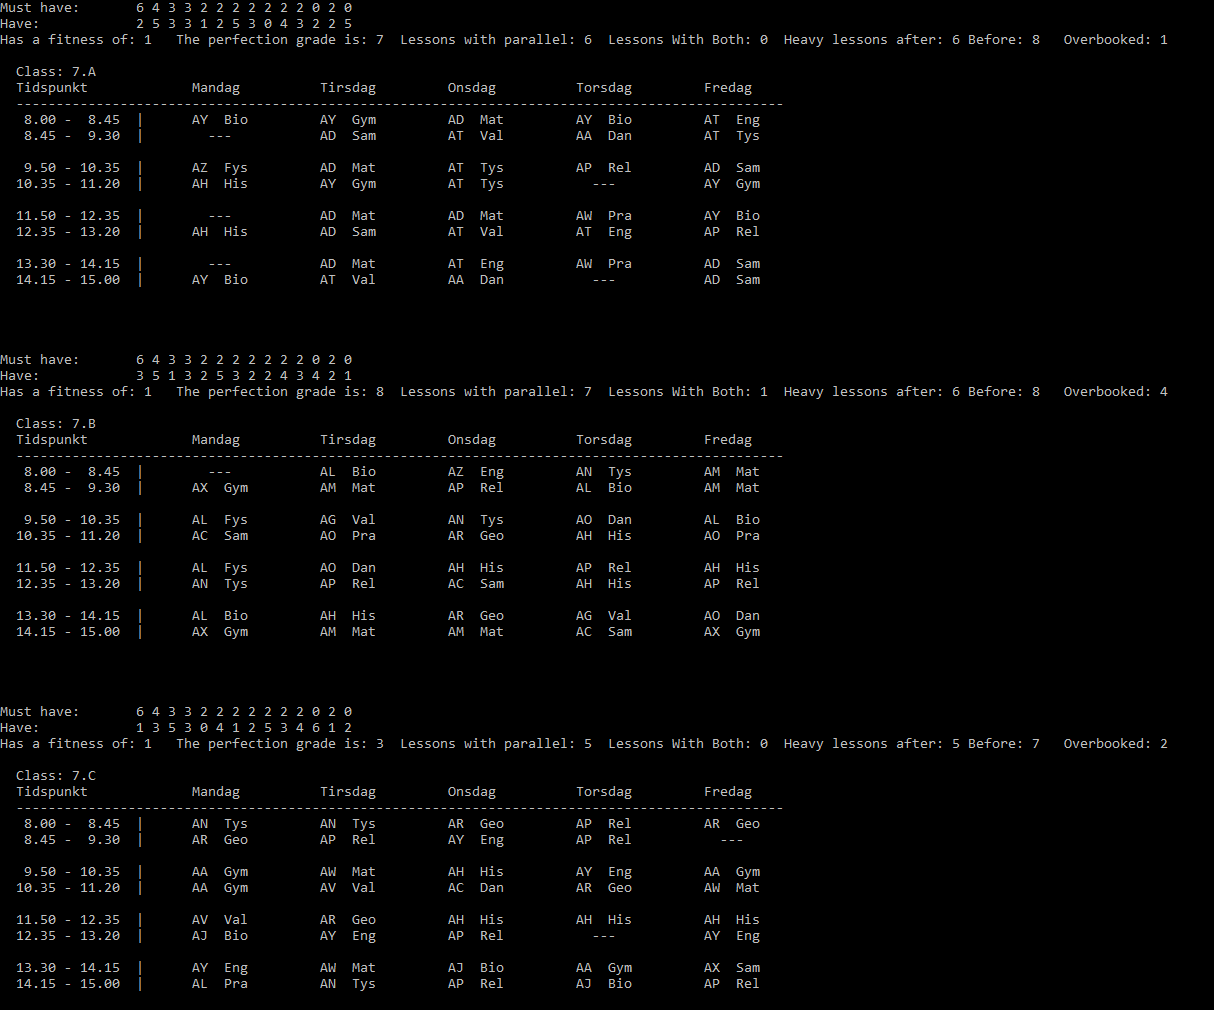
\includegraphics[width=\textwidth]{partials/graphics/startsskema.png}
  \caption{Genereret udkast af skemaer til 7.a, b og c }
  \label{fig:startsskema}
\end{figure}